\documentclass[main.tex]{subfiles}
\begin{document}
	
Python 有好几种免费的,且功能卓越的集成开发环境(IDE - Integrated Development Environment)软件。《数学:编程与作图》一书采用的是包括在
Anaconda Navigator  套装里的 Spyder。Spyder 同时提供 Python 的代码编辑、交互运行和图形绘制的开发平台。包括在 Anaconda Navigator 里的 Jupyter 也提供这样的开发平台。包括在 Anaconda Navigator 里的 VS Code (Microsoft Visual Studio Code) 虽然也是比较受欢迎的,并支持包括 Python 在内的多语言 IDE,但一些常用的 Python 包和库需要另行安装和配置,我们就不作进一步介绍。免费的、专业开发人员中受欢迎的 IntelliJ Community 版本也存在这个问题。

下面介绍 Anaconda Navigator 的安装步骤。

1、访问网址:\texttt{https://www.anaconda.com}(图\ref{fig:1.1})。

\begin{figure}[h]
	\centering
	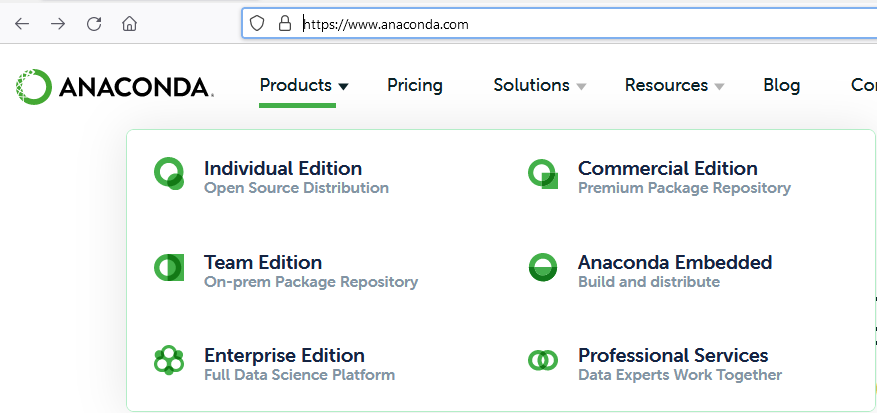
\includegraphics[width=1.0\textwidth]{anaconda_home.png}
	\caption{访问 Anaconda Navigator 网址}
	\label{fig:1.1}
\end{figure}

2、个人版本(Individual Edition)是免费的。点击链接 Individual Edition  后,显示(图 \ref{fig:1.2}),到达

\texttt{https://www.anaconda.com/products/individual}。

\begin{figure}[h]
	\centering
	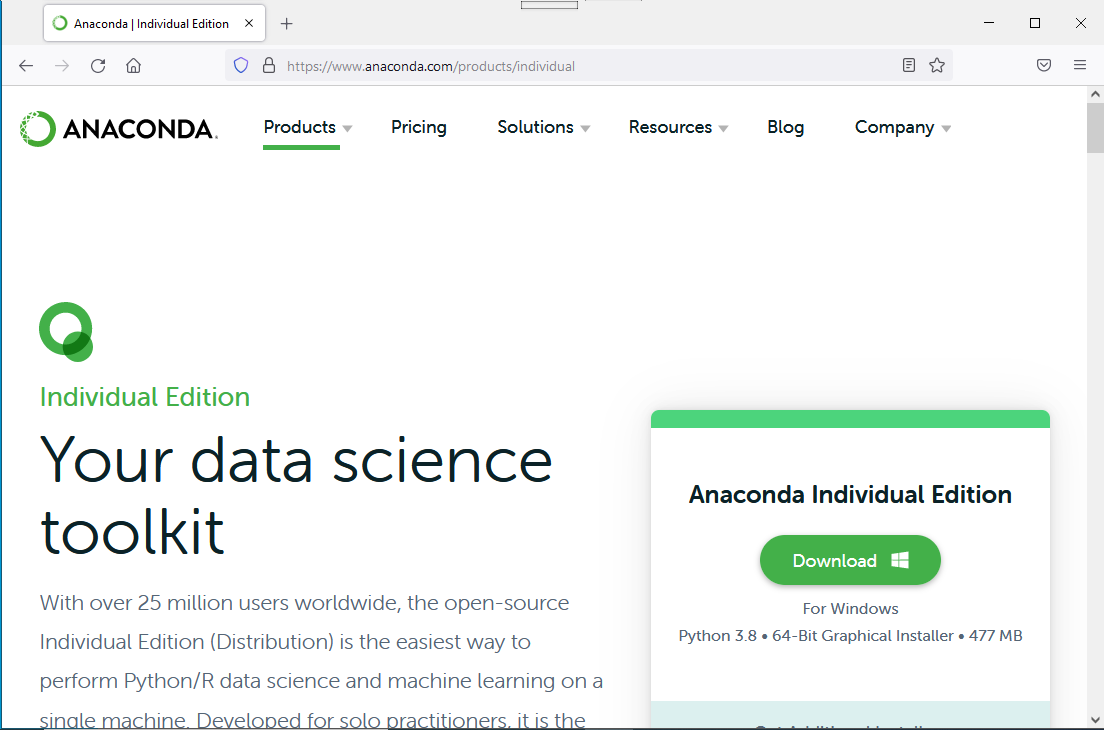
\includegraphics[width=1.0\textwidth]{anaconda_download.png}
	\caption{访问 Anaconda Navigator 网址}
	\label{fig:1.2}
\end{figure}

滚动到显示 Anaconda 个人版本下载按钮(Anaconda Individual Edition Download)的地方。如果操作系统是视窗,则有 For Windows 的字样。如果操作系统是MacBook,则有 For MacOS 的字样。

\newpage
3、点击 Download,则见对话框(图 \ref{fig:1.3})。
\begin{figure}[b]
	\centering
	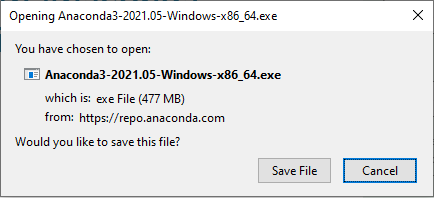
\includegraphics[scale=1]{anaconda_download_file.png}
	\caption{访问 Anaconda Navigator 网址}
	\label{fig:1.3}
\end{figure}


\verb|https://www.spyder-ide.org|

Python software installation:



微软公司的视窗操作系统的主要开发语言是C\#,其 IDE 是 Microsoft Visual Studio ${}^{\textregistered}$。但他们也有一个免费的轻巧 IDE,叫做 Visual Studio Code,有 Windows, Linux and macOS 版本,支持 Python,Java,JavaScript,Go,Node.js 和 C++ 等语言。可从
https://code.visualstudio.com
下载的安装。


\end{document} 
